% Options for packages loaded elsewhere
\PassOptionsToPackage{unicode}{hyperref}
\PassOptionsToPackage{hyphens}{url}
\documentclass[
  ignorenonframetext,
]{beamer}
\newif\ifbibliography
\usepackage{pgfpages}
\setbeamertemplate{caption}[numbered]
\setbeamertemplate{caption label separator}{: }
\setbeamercolor{caption name}{fg=normal text.fg}
\beamertemplatenavigationsymbolsempty
% remove section numbering
\setbeamertemplate{part page}{
  \centering
  \begin{beamercolorbox}[sep=16pt,center]{part title}
    \usebeamerfont{part title}\insertpart\par
  \end{beamercolorbox}
}
\setbeamertemplate{section page}{
  \centering
  \begin{beamercolorbox}[sep=12pt,center]{section title}
    \usebeamerfont{section title}\insertsection\par
  \end{beamercolorbox}
}
\setbeamertemplate{subsection page}{
  \centering
  \begin{beamercolorbox}[sep=8pt,center]{subsection title}
    \usebeamerfont{subsection title}\insertsubsection\par
  \end{beamercolorbox}
}
% Prevent slide breaks in the middle of a paragraph
\widowpenalties 1 10000
\raggedbottom
\AtBeginPart{
  \frame{\partpage}
}
\AtBeginSection{
  \ifbibliography
  \else
    \frame{\sectionpage}
  \fi
}
\AtBeginSubsection{
  \frame{\subsectionpage}
}
\usepackage{iftex}
\ifPDFTeX
  \usepackage[T1]{fontenc}
  \usepackage[utf8]{inputenc}
  \usepackage{textcomp} % provide euro and other symbols
\else % if luatex or xetex
  \usepackage{unicode-math} % this also loads fontspec
  \defaultfontfeatures{Scale=MatchLowercase}
  \defaultfontfeatures[\rmfamily]{Ligatures=TeX,Scale=1}
\fi
\usepackage{lmodern}
\ifPDFTeX\else
  % xetex/luatex font selection
\fi
% Use upquote if available, for straight quotes in verbatim environments
\IfFileExists{upquote.sty}{\usepackage{upquote}}{}
\IfFileExists{microtype.sty}{% use microtype if available
  \usepackage[]{microtype}
  \UseMicrotypeSet[protrusion]{basicmath} % disable protrusion for tt fonts
}{}
\makeatletter
\@ifundefined{KOMAClassName}{% if non-KOMA class
  \IfFileExists{parskip.sty}{%
    \usepackage{parskip}
  }{% else
    \setlength{\parindent}{0pt}
    \setlength{\parskip}{6pt plus 2pt minus 1pt}}
}{% if KOMA class
  \KOMAoptions{parskip=half}}
\makeatother
\usepackage{color}
\usepackage{fancyvrb}
\newcommand{\VerbBar}{|}
\newcommand{\VERB}{\Verb[commandchars=\\\{\}]}
\DefineVerbatimEnvironment{Highlighting}{Verbatim}{commandchars=\\\{\}}
% Add ',fontsize=\small' for more characters per line
\usepackage{framed}
\definecolor{shadecolor}{RGB}{248,248,248}
\newenvironment{Shaded}{\begin{snugshade}}{\end{snugshade}}
\newcommand{\AlertTok}[1]{\textcolor[rgb]{0.94,0.16,0.16}{#1}}
\newcommand{\AnnotationTok}[1]{\textcolor[rgb]{0.56,0.35,0.01}{\textbf{\textit{#1}}}}
\newcommand{\AttributeTok}[1]{\textcolor[rgb]{0.13,0.29,0.53}{#1}}
\newcommand{\BaseNTok}[1]{\textcolor[rgb]{0.00,0.00,0.81}{#1}}
\newcommand{\BuiltInTok}[1]{#1}
\newcommand{\CharTok}[1]{\textcolor[rgb]{0.31,0.60,0.02}{#1}}
\newcommand{\CommentTok}[1]{\textcolor[rgb]{0.56,0.35,0.01}{\textit{#1}}}
\newcommand{\CommentVarTok}[1]{\textcolor[rgb]{0.56,0.35,0.01}{\textbf{\textit{#1}}}}
\newcommand{\ConstantTok}[1]{\textcolor[rgb]{0.56,0.35,0.01}{#1}}
\newcommand{\ControlFlowTok}[1]{\textcolor[rgb]{0.13,0.29,0.53}{\textbf{#1}}}
\newcommand{\DataTypeTok}[1]{\textcolor[rgb]{0.13,0.29,0.53}{#1}}
\newcommand{\DecValTok}[1]{\textcolor[rgb]{0.00,0.00,0.81}{#1}}
\newcommand{\DocumentationTok}[1]{\textcolor[rgb]{0.56,0.35,0.01}{\textbf{\textit{#1}}}}
\newcommand{\ErrorTok}[1]{\textcolor[rgb]{0.64,0.00,0.00}{\textbf{#1}}}
\newcommand{\ExtensionTok}[1]{#1}
\newcommand{\FloatTok}[1]{\textcolor[rgb]{0.00,0.00,0.81}{#1}}
\newcommand{\FunctionTok}[1]{\textcolor[rgb]{0.13,0.29,0.53}{\textbf{#1}}}
\newcommand{\ImportTok}[1]{#1}
\newcommand{\InformationTok}[1]{\textcolor[rgb]{0.56,0.35,0.01}{\textbf{\textit{#1}}}}
\newcommand{\KeywordTok}[1]{\textcolor[rgb]{0.13,0.29,0.53}{\textbf{#1}}}
\newcommand{\NormalTok}[1]{#1}
\newcommand{\OperatorTok}[1]{\textcolor[rgb]{0.81,0.36,0.00}{\textbf{#1}}}
\newcommand{\OtherTok}[1]{\textcolor[rgb]{0.56,0.35,0.01}{#1}}
\newcommand{\PreprocessorTok}[1]{\textcolor[rgb]{0.56,0.35,0.01}{\textit{#1}}}
\newcommand{\RegionMarkerTok}[1]{#1}
\newcommand{\SpecialCharTok}[1]{\textcolor[rgb]{0.81,0.36,0.00}{\textbf{#1}}}
\newcommand{\SpecialStringTok}[1]{\textcolor[rgb]{0.31,0.60,0.02}{#1}}
\newcommand{\StringTok}[1]{\textcolor[rgb]{0.31,0.60,0.02}{#1}}
\newcommand{\VariableTok}[1]{\textcolor[rgb]{0.00,0.00,0.00}{#1}}
\newcommand{\VerbatimStringTok}[1]{\textcolor[rgb]{0.31,0.60,0.02}{#1}}
\newcommand{\WarningTok}[1]{\textcolor[rgb]{0.56,0.35,0.01}{\textbf{\textit{#1}}}}
\usepackage{graphicx}
\makeatletter
\newsavebox\pandoc@box
\newcommand*\pandocbounded[1]{% scales image to fit in text height/width
  \sbox\pandoc@box{#1}%
  \Gscale@div\@tempa{\textheight}{\dimexpr\ht\pandoc@box+\dp\pandoc@box\relax}%
  \Gscale@div\@tempb{\linewidth}{\wd\pandoc@box}%
  \ifdim\@tempb\p@<\@tempa\p@\let\@tempa\@tempb\fi% select the smaller of both
  \ifdim\@tempa\p@<\p@\scalebox{\@tempa}{\usebox\pandoc@box}%
  \else\usebox{\pandoc@box}%
  \fi%
}
% Set default figure placement to htbp
\def\fps@figure{htbp}
\makeatother
\setlength{\emergencystretch}{3em} % prevent overfull lines
\providecommand{\tightlist}{%
  \setlength{\itemsep}{0pt}\setlength{\parskip}{0pt}}
\usepackage{bookmark}
\IfFileExists{xurl.sty}{\usepackage{xurl}}{} % add URL line breaks if available
\urlstyle{same}
\hypersetup{
  pdftitle={TMA4315 Generalized linear models H2018},
  pdfauthor={Mette Langaas, Department of Mathematical Sciences, NTNU -- with contributions from Ingeborg Hem},
  hidelinks,
  pdfcreator={LaTeX via pandoc}}

\title{TMA4315 Generalized linear models H2018}
\subtitle{Module 4: Count and continuous positive response data (Poisson
and gamma regression)}
\author{Mette Langaas, Department of Mathematical Sciences, NTNU -- with
contributions from Ingeborg Hem}
\date{27.09.2018 and 04.10.2018 {[}PL{]}, 28.09.2018 and 05.10.2018
{[}IL{]}}

\begin{document}
\frame{\titlepage}

\begin{frame}
(Latest changes: 06.10: solutions added. 01.10: small changes for second
week. 27.09: added one Problem for ILw1, moved stuff to w2, added a few
dimensions to score test.)
\end{frame}

\begin{frame}{Overview}
\phantomsection\label{overview}
\begin{block}{Learning material}
\phantomsection\label{learning-material}
\begin{itemize}
\tightlist
\item
  Textbook: Fahrmeir et al (2013): Chapter 5.2, 5.3.
\item
  \href{https://www.math.ntnu.no/emner/TMA4315/2018h/TMA4315M4H20180927.pdf}{Classnotes
  27.09.2018}
\item
  \href{https://www.math.ntnu.no/emner/TMA4315/2018h/TMA4315M4H20181004.pdf}{Classnotes
  04.10.2018}
\end{itemize}
\end{block}
\end{frame}

\begin{frame}
\begin{block}{Topics}
\phantomsection\label{topics}
\begin{block}{\hyperlink{firstweek}{First week}}
\phantomsection\label{first-week}
\begin{itemize}
\tightlist
\item
  examples of count data
\item
  the Poisson distribution
\item
  regression with count data
\item
  Poisson regression with log-link
\item
  parameter estimation (ML): log-likelhood, score vector, information
  matrix to give iterative calculations
\item
  asymptotic MLE properties
\item
  confidence intervals and hypothesis tests (Wald, score and LRT)
\end{itemize}
\end{block}
\end{block}
\end{frame}

\begin{frame}
\begin{block}{\hyperlink{secondweek}{Second week}}
\phantomsection\label{second-week}
\begin{itemize}
\item
  Count data with Poisson regression (continued)
\item
  deviance, model fit and model choice
\item
  overdispersion
\item
  rate models and offset
\item
  Modelling continuous response data: lognormal and gamma
\item
  the gamma distribution
\item
  the gamma GLM model
\item
  gamma likelihood and derivations thereof
\item
  dispersion parameter: scaled and unscaled deviance
\end{itemize}
\end{block}
\end{frame}

\begin{frame}
\textbf{FIRST WEEK}
\end{frame}

\begin{frame}{Examples of count data}
\phantomsection\label{examples-of-count-data}
\begin{itemize}
\tightlist
\item
  the number of automobile thefts pr city worldwide
\item
  the number of UFO sightings around the world
\item
  the number of visits at web pages
\item
  the number of male crabs (satellites) residing nearby a female crab
\item
  the number of goals by the home team and the number of goals for the
  away team in soccer
\item
  the number of newspapers sold at newsagents
\item
  the number of vampires living on Sesame Street
\end{itemize}
\end{frame}

\begin{frame}
\begin{block}{Sales of newspapers}
\phantomsection\label{sales-of-newspapers}
Response data: number of newspapers (delivered) sold at each outlet.
Covariate data: type of outlet, but mainly calendar information=
weekday, month, season, public holidays, winter/autumn/easter/xmas,
\ldots{}

The aim: predict the number of newspapers sold at each oulet (11,000!)
in Norway on any day

Can use this to optimise the number of newspapers printed and delivered
\end{block}
\end{frame}

\begin{frame}[fragile]
\begin{block}{Female horseshoe crabs with satellites}
\phantomsection\label{female-horseshoe-crabs-with-satellites}
The study objects were female horseshoe crabs. Each female horseshoe
crab had a male attached to her in her nest. The objective of the study
was to investigate factors that affect whether the female had any other
males, called satellites, residing near her. The following covariates
were collected for 173 female horseshoe crabs:

\begin{itemize}
\tightlist
\item
  \texttt{C}: the color of the female horseshoe crab (1=light medium,
  2=medium, 3=dark medium, 4=dark)
\item
  \texttt{S}: spine condition (1=both good, 2=one worn or broken, 3=both
  worn or broken)
\item
  \texttt{W}: width of carapace (cm)
\item
  \texttt{Wt}: weight (kg)
\end{itemize}

The response was the number of satellites, \texttt{Sa} = male horseshoe
crabs residing nearby.
\end{block}
\end{frame}

\begin{frame}[fragile]
\pandocbounded{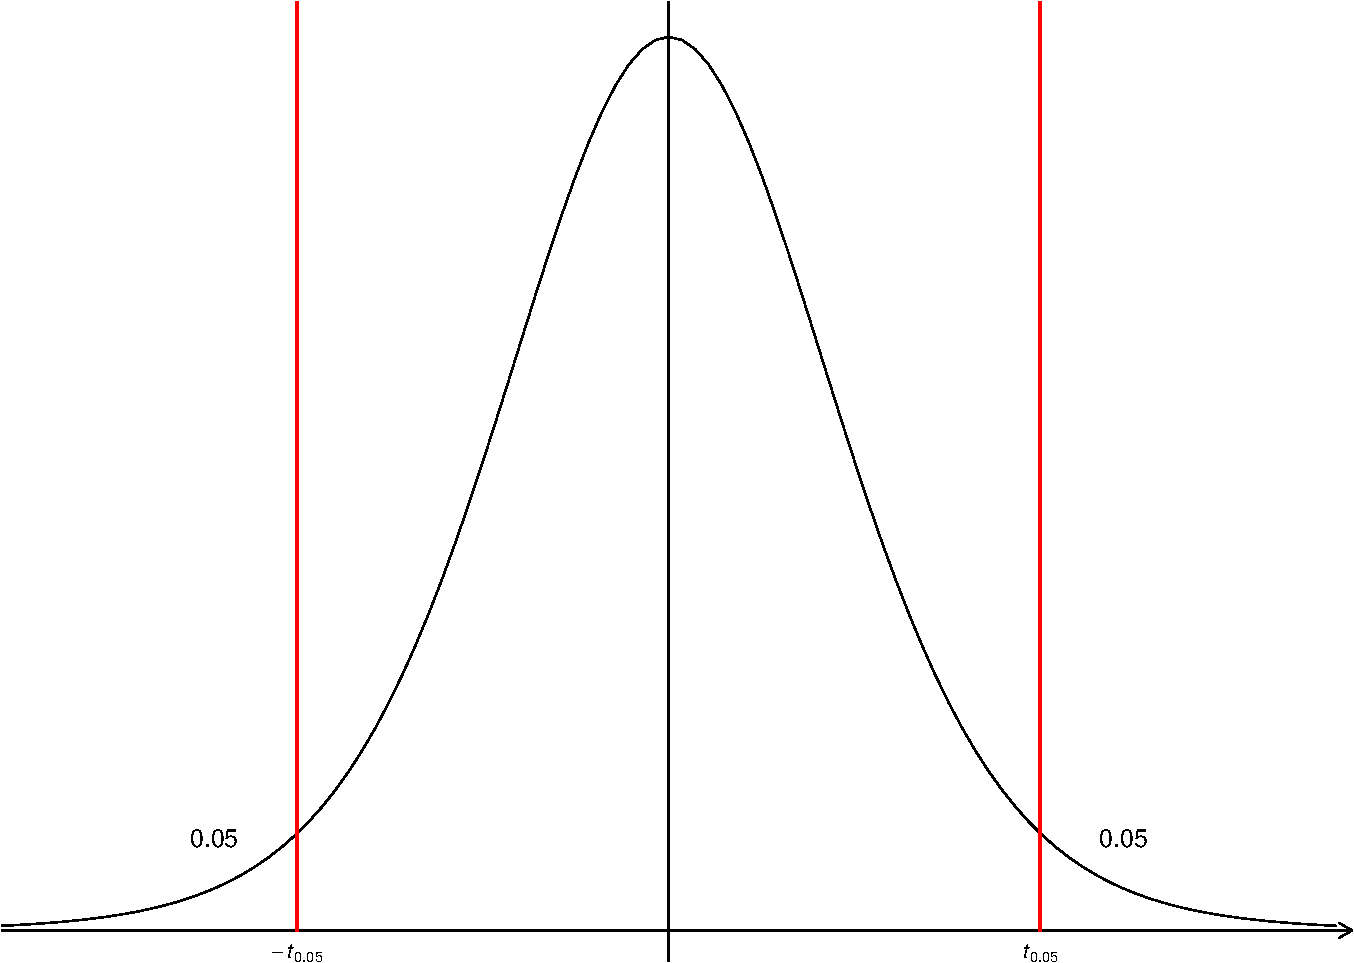
\includegraphics[keepaspectratio]{Module04PoissonGammaPresentationWeek1_files/figure-beamer/unnamed-chunk-1-1.pdf}}

\textbf{Q}: Discuss what you see. Any potential covariates to influence
\texttt{Sa}? Which distribution can \texttt{Sa} have?
\end{frame}

\begin{frame}{Modelling counts with the Poisson distribution}
\phantomsection\label{modelling-counts-with-the-poisson-distribution}
\begin{block}{The Poisson process}
\phantomsection\label{the-poisson-process}
We observe events that may occur within a time interval or a region.

\begin{enumerate}
\tightlist
\item
  The number of events occuring within a time interval or a region, is
  independent of the number of events that occurs in any other disjoint
  (non-overlapping) time interval or region.
\item
  The probability that a single event occurs within a small time
  interval or region, is proportional to the length of the interval or
  the size of the region.
\item
  The probability that more than one event may occur within a small time
  interval or region is negligible.
\end{enumerate}
\end{block}
\end{frame}

\begin{frame}
When all of these three properties are fulfilled we have a \emph{Poisson
process}. This leads to three distributions

\begin{itemize}
\tightlist
\item
  The number of events in a Poisson process follows a Poisson
  distribution.
\item
  Time between two events in a Poisson process follows an exponential
  distribution.
\item
  Time between many events in a Poisson process follows a gamma
  distribution.
\end{itemize}

We will first study the Poisson distribution - and link it to a
regression setting.
\end{frame}

\begin{frame}[fragile]
\begin{block}{The Poisson distribution}
\phantomsection\label{the-poisson-distribution}
We study a Poisson process within a time interval or a region of
specified size. Then, the number of events, \(Y\), will follow a
\emph{Poisson distribution} with parameter \(\lambda\)

\[
f(y)=\frac{\lambda^y}{y!}e^{-\lambda} \text{ for } y=0,1,2,…
\] Here the parameter \(\lambda\) is the proportionality factor in the
requirement 2 (above) for the Poisson process. Another popular
parameterization is \(\mu\), or given some interval \(\lambda t\), but
we will stick with \(\lambda\). In R we calculate the Poisson point
probabilities using \texttt{dpois}.
\end{block}
\end{frame}

\begin{frame}
\begin{block}{Expected value and variance}
\phantomsection\label{expected-value-and-variance}
Let \(Y\) follow a Poisson distribution with parameter \(\lambda\). Then
\[\text{E}(Y)=\lambda \text{ and } \text{Var}(Y)=\lambda\] (proofs in
notes)
\end{block}
\end{frame}

\begin{frame}
\begin{block}{Properties of the Poisson distribution}
\phantomsection\label{properties-of-the-poisson-distribution}
\begin{itemize}
\tightlist
\item
  A sum of \(n\) independent Poisson distributed random variables,
  \(Y_i\) with means \(\lambda_i\) are Poisson distributed with mean
  \(\sum_{i=1}^n \lambda_i\).
\item
  When the mean increases the Poisson distribution becomes more and more
  symmetric and for large \(\lambda\) the Poisson distribution can be
  approximated by a normal distribution.
\end{itemize}
\end{block}
\end{frame}

\begin{frame}
\begin{block}{Exponential family}
\phantomsection\label{exponential-family}
In Module 1 we introduced distributions of the \(Y_i\), that could be
written in the form of a \emph{univariate exponential family}

\[ 
f(y_i\mid \theta_i)=\exp \left( \frac{y_i \theta_i-b(\theta_i)}{\phi}\cdot w_i + c(y_i, \phi, w_i) \right)
\] where we said that

\begin{itemize}
\tightlist
\item
  \(\theta_i\) is called the canonical parameter and is a parameter of
  interest
\item
  \(\phi\) is called a nuisance parameter (and is not of interest to
  us=therefore a nuisance (plage))
\item
  \(w_i\) is a weight function, in most cases \(w_i=1\)
\item
  \(b\) and \(c\) are known functions.
\end{itemize}
\end{block}
\end{frame}

\begin{frame}
\begin{block}{Exponentially Poisson}
\phantomsection\label{exponentially-poisson}
The log- likelihood for a Poisson is

\[l(\theta)=\ln L(\theta)=\sum_{i=1}^n \ln L_i(\beta)=\sum_{i=1}^n l_i(\beta)=\sum_{i=1}^n [y_i \ln(\lambda_i)-\lambda_i-\ln(y!)]\]
So, comparing with

\[ 
l(\theta_i; y_i)=\frac{y_i \theta_i-b(\theta_i)}{\phi}\cdot w_i + c(y_i, \phi, w_i)
\]

we get

\begin{itemize}
\tightlist
\item
  \(\theta_i=\ln(\lambda_i)\) is the canonical parameter
\item
  \(\phi=1\), no nuisance
\item
  \(w_i=1\)
\item
  \(b(\theta_i)=\exp(\theta)\)
\item
  \(\mu_i=\text{E}(Y_i)=\lambda_i\)
\end{itemize}
\end{block}
\end{frame}

\begin{frame}
For a GLM with linear predictor \(\eta_i\) - to have a canonical link we
need \[\theta_i=\eta_i\] Since \(\eta_i=g(\mu_i)=g(\lambda_i)\) this
means to us that we need \[ g(\mu_i)=g(\lambda_i)=\theta_i\] saying that
with the Poisson the canonical link is \(\ln(\lambda_i)\).

\textbf{Q}: Why may we want to choose a canonical link?
\end{frame}

\begin{frame}{Regression with count data}
\phantomsection\label{regression-with-count-data}
\begin{block}{Aim}
\phantomsection\label{aim}
\begin{enumerate}
\item
  Construct a model to help understand the relationship between a count
  variable and one or many possible explanatory variables. The response
  measurements are counts.
\item
  Use the model for understanding what can explain count, and for
  prediction of counts.
\end{enumerate}

(you can use OLS, but you might have to transform the response to
stabilise the variance. If the counts are all large, OLS will work fine)
\end{block}
\end{frame}

\begin{frame}
\begin{block}{The log-linear Poisson model}
\phantomsection\label{the-log-linear-poisson-model}
\textbf{Assumptions: }

\begin{enumerate}
\item
  \(Y_i \sim \text{Poisson}(\lambda_i)\), with
  \(\text{E}(Y_i)=\lambda_i\), and \(\text{Var}(Y_i)=\lambda_i\).
\item
  Linear predictor: \(\eta_i={\bf x}_i^T \beta\).
\item
  Log link \[\eta_i=\ln(\lambda_i)=g(\lambda_i)\] and (inverse thereof)
  response function \[\lambda_i=\exp(\eta_i)\]
\end{enumerate}

Assumptions 1 and 3 above can be written as
\[Y_i \sim \text{Poisson}(\exp(\eta_i)), \text{ }i=1,\ldots,n\]
\end{block}
\end{frame}

\begin{frame}
\begin{block}{Interpreting parameters in the log-linear Poisson model}
\phantomsection\label{interpreting-parameters-in-the-log-linear-poisson-model}
In the log-linear model the mean, \(\text{E}(Y_i)=\lambda_i\) satisfy an
exponential relationship to covariates
\[ \lambda_i=\exp(\eta_i)=\exp({\bf x}_i^T \beta)=\exp(\beta_0)\cdot \exp(\beta_1)^{x_{i1}}
\cdots \exp(\beta_k)^{x_{ik}}.\]

Let us look in detail at \(\beta_1\) with covariate \(x_{i1}\) for
observation \(i\).

\begin{enumerate}
\tightlist
\item
  If \(x_{i1}\) increases by one unit to \(x_{i1}+1\) then the mean
  \(\text{E}(Y_i)\) will in our model change by a factor
  \(\exp(\beta_1)\).
\item
  If \(\beta_1\)=0 then \(\exp(\beta_1)=1\), so that a change in
  \(x_{i1}\) does not change \(\text{E}(Y_i)\).
\item
  If \(\beta_1<0\) then \(\exp(\beta_1)<1\) so if \(x_{i1}\) increase
  then \(\text{E}(Y_i)\) decrease.
\item
  If \(\beta_1>0\) then \(\exp(\beta_1)>1\) so if \(x_{i1}\) increase
  then \(\text{E}(Y_i)\) increase.
\end{enumerate}

Thus, the covariates have a multiplicative effect on the rate
\(\lambda_i\).
\end{block}
\end{frame}

\begin{frame}[fragile]
\begin{block}{Example: interpreting parameters for the female crabs with
satellites}
\phantomsection\label{example-interpreting-parameters-for-the-female-crabs-with-satellites}
We fit a log-linear model to \texttt{Sa}, assuming the number of
satellites follows a Poisson distribution with log-link, and use S
(spine condition) as a covariate.

\begin{verbatim}
## Intercept + 
## (Intercept)          S2          S3 
##   1.2943569  -0.6012097  -0.2612018 
## Intercept+W, exp
## (Intercept)          S2          S3 
##   3.6486486   0.5481482   0.7701255
\end{verbatim}

(1=both good, 2=one worn or broken, 3=both worn or broken)

So S2 roughly halves the number of satellite males
\end{block}
\end{frame}

\begin{frame}{Parameter estimation with maximum likelihood}
\phantomsection\label{parameter-estimation-with-maximum-likelihood}
We would like to estimate \(\beta\) by maximizing the likelihood -

This is essentially the same as for Module 3: Binary regression - with
``Poisson and log'' instead of ``Bernoulli and logit''.
\end{frame}

\begin{frame}
\begin{block}{Likelihood \(L(\beta)\)}
\phantomsection\label{likelihood-lbeta}
We assume that pairs of covariates and response are measured
independently of each other: \(({\bf x}_i,Y_i)\), and \(Y_i\) follows
the distribution specified above, and \({\bf x}_i\) is fixed.

\[L(\beta)=\prod_{i=1}^n L_i(\beta)=\prod_{i=1}^n f(y_i; \beta)=\prod_{i=1}^n\frac{\lambda_i^{y_i}}{y_i!}\exp(-\lambda_i)\]

\textbf{Note:} still a slight misuse of notation - where is \(\beta\)?
\end{block}
\end{frame}

\begin{frame}
\begin{block}{Loglikelihood \(l(\beta)\)}
\phantomsection\label{loglikelihood-lbeta}
\[l(\beta)=\ln L(\beta)=\sum_{i=1}^n \ln L_i(\beta)=\sum_{i=1}^n l_i(\beta)=\sum_{i=1}^n [y_i \ln(\lambda_i)-\lambda_i-\ln(y!)]\]
Observe that the log-likelihood is a sum of individual contributions for
each observation pair \(i\). We often omit the last term since it is not
a function of model parameters, only data.
\end{block}
\end{frame}

\begin{frame}
If we want a function of \(\eta_i=\ln(\lambda_i)\) or \(\beta\):
\[l(\beta)=\sum_{i=1}^n[y_i \eta_i-\exp(\eta_i)+C_i]=\sum_{i=1}^n y_i{\bf x}_i^T\beta-\sum_{i=1}^n  \exp({\bf x}_i^T\beta) +C\]
\end{frame}

\begin{frame}
\begin{block}{Score function \(s(\beta)\)}
\phantomsection\label{score-function-sbeta}
The score function is a \(p\times 1\) vector, \(s(\beta)\), with the
partial derivatives of the log-likelihood with respect to the \(p\)
elements of the \(\beta\) vector. Remember, the score function is linear
in the individual contributions:
\[s(\beta)=\frac{\partial l(\beta)}{\partial \beta}=
\sum_{i=1}^n \frac{\partial l_i(\beta)}{\partial \beta}=
\sum_{i=1}^n s_i(\beta)\]

We use the chain rule to find \(s_i(\beta)\).

\[
\begin{aligned}
s_i(\beta)&=\frac{\partial l_i(\beta)}{\partial \beta}=\frac{\partial l_i(\beta)}{\partial \eta_i}\cdot \frac{\partial \eta_i}{\partial \beta} \\
&=\frac{\partial [y_i\eta_i-\exp(\eta_i)+C_i]}{\partial \eta_i}\cdot \frac{\partial [{\bf x}_i^T\beta ]}{\partial \beta}\\
&=[y_i-\exp(\eta_i)]\cdot {\bf x}_i \\
&=(y_i-\lambda_i){\bf x}_i
\end{aligned}
\]

(see Module 3 for rules for partial derivatives of scalar wrt vector)
\end{block}
\end{frame}

\begin{frame}
The score function is given as:

\[s(\beta)=\sum_{i=1}^n s_i(\beta)=\sum_{i=1}^n (y_i-\lambda_i){\bf x}_i\]
So

\[
\text{E}(s_i(\beta))=\text{E}((Y_i-\lambda_i){\bf x}_i)=0
\]

(because \(\text{E}(Y_i)=\lambda_i\), thus \(\text{E}(s(\beta))=0\)).
\end{frame}

\begin{frame}
\begin{block}{Fisher Information}
\phantomsection\label{fisher-information}
We will also need the Fisher Information, for the estimation (=a
numerical optimisation problem), and to estimate the covariances

\begin{itemize}
\tightlist
\item
  the \textbf{expected} Fisher information matrix,
  \(F(\beta) = \text{Cov}(\beta)\)
\item
  the \textbf{observed} Fisher information matrix,
  \(H(\beta) = -{\partial s(\beta)}/{\partial\beta^T}\)
\item
  for us \(F(\beta) = H(\beta)\)
\end{itemize}
\end{block}
\end{frame}

\begin{frame}
\begin{block}{The expected Fisher information matrix \(F(\beta)\)}
\phantomsection\label{the-expected-fisher-information-matrix-fbeta}
\[
F(\beta) = \text{Cov}(s(\beta)) = \sum_{i=1}^n \text{Cov}(s_i(\beta)) = \dots = \sum_{i=1}^n F_i(\beta) 
\]

assuming the responses \(Y_i\) and \(Y_j\) are independent, and that
\(E(s_i(\beta)) = 0 \ \forall i\).

Remember that \(s_i(\beta)=(Y_i-\lambda_i){\bf x}_i\), then:

\[
\begin{aligned}
F_i(\beta) &= E(s_i(\beta)s_i(\beta)^T) = E((Y_i-\lambda_i){\bf x}_i(Y_i-\lambda_i){\bf x}_i^T)\\
&= {\bf x}_i{\bf x}_i^T E((Y_i-\lambda_i)^2) \\
&= {\bf x}_i{\bf x}_i^T \lambda_i
\end{aligned}
\] where \(E((Y_i-\lambda_i)^2)=\text{Var}(Y_i)=\lambda\) is the
variance of \(Y_i\). Thus

\[F(\beta) = \sum_{i=1}^n {\bf x}_i{\bf x}_i^T \lambda_i.\]
\end{block}
\end{frame}

\begin{frame}
\begin{block}{Observed Fisher information matrix \(H(\beta)\)}
\phantomsection\label{observed-fisher-information-matrix-hbeta}
Since we use canonical link \(H(\beta)=F(\beta)\). But, for
completeness, we add the direct derivation of \(H(\beta)\).

\[
\begin{aligned}
H(\beta) &= -\frac{\partial^2l(\beta)}{\partial\beta\partial\beta^T} = -\frac{\partial s(\beta)}{\partial\beta^T} \\
&= \frac{\partial}{\partial\beta^T}\left[\sum_{i=1}^n (\lambda_i-y_i){\bf x}_i \right] \;\; (s(\beta) = \sum_{i=1}^n (y_i-\lambda_i){\bf x}_i)\\
&=\frac{\partial}{\partial\beta^T}\left[\sum_{i=1}^n (\exp(\eta_i)-y_i){\bf x}_i \right] \;\; (\lambda_i = \exp(\eta_i))
\end{aligned}
\]
\end{block}
\end{frame}

\begin{frame}
\[H(\beta) = \sum_{i=1}^n \frac{\partial}{\partial\beta^T}[{\bf x}_i\lambda_i-{\bf x}_iy_i] = \sum_{i=1}^n \frac{\partial}{\partial\beta^T}{\bf x}_i\lambda_i = \sum_{i=1}^n {\bf x}_i \frac{\partial \lambda_i}{\partial \eta_i} \frac{\partial \eta_i}{\partial \beta^T} \]

Use that

\[ \frac{\partial \eta_i}{\partial \beta^T}=\frac{\partial {\bf x}_i^T\beta}{\partial \beta^T} = \left(\frac{\partial {\bf x}_i^T\beta}{\partial \beta}\right)^T = {\bf x}_i^T \]

and

\[ \frac{\partial \lambda_i}{\partial \eta_i} =  \frac{\partial\exp(\eta_i)}{\partial \eta_i} = \exp(\eta_i)=\lambda_i\]

And thus

\[H(\beta) =\sum_{i=1}^n {\bf x}_i {\bf x}_i^T\lambda_i.\]
\end{frame}

\begin{frame}
\begin{block}{How to solve it}
\phantomsection\label{how-to-solve-it}
To find the maximum likelihood estimate \(\hat{\beta}\) we solve the set
of \(p\) non-linear equations: \[s(\hat{\beta})=0\] And, as before we do
that using the Newton-Raphson or Fisher Scoring iterative methods, so we
need the derivative of the score vector (our Fisher information).
\end{block}
\end{frame}

\begin{frame}{Parameter estimation - in practice}
\phantomsection\label{parameter-estimation---in-practice}
To find the ML estimate \(\hat{\beta}\) we need to solve
\[s(\hat{\beta})=0\] We have that the score function for the log-linear
model is:
\[s(\beta)=\sum_{i=1}^n {\bf x}_i (y_i-\lambda_i)=\sum_{i=1}^n {\bf x}_i (y_i-\exp({\bf x}_i^T\beta)).\]
Observe that this is a non-linear function in \(\beta\), and has no
closed form solution (except for a few special cases).
\end{frame}

\begin{frame}
\begin{block}{Fisher scoring}
\phantomsection\label{fisher-scoring}
To solve this we use the Fisher scoring algorithm, were we at interation
\(t+1\) have

\[\beta^{(t+1)}=\beta^{(t)} + F(\beta^{(t)})^{-1} s(\beta^{(t)})\]

Remark: what do we need to do to use the Newton-Raphson method instead?
Well, replace \(F\) with \(H\), but for canonical link (which is the
log-link for the Poisson) \(F=H\).
\end{block}
\end{frame}

\begin{frame}
\begin{block}{Requirements for convergence}
\phantomsection\label{requirements-for-convergence}
For the Fisher scoring algorithm the expected Fisher information matrix
\(F\) needs to be invertible. For this we need:

\begin{itemize}
\tightlist
\item
  \(\lambda_i>0\) for all \(i\)
\item
  design matrix (\(X\))has full rank (\(p\)).
\end{itemize}

For the log link \(\lambda_i=\exp({\bf x}_i^T\beta)\) which is always
positive.

Note, with the linear link \(\lambda_i=\eta_i\) this might be a
challenge, and restrictions on \(\beta\) must be set.

The algorithm might not converge, if the data are evil enough,
particularly with small samples.
\end{block}
\end{frame}

\begin{frame}{Statistical inference}
\phantomsection\label{statistical-inference}
\begin{block}{Asymptotic properties of ML estimates}
\phantomsection\label{asymptotic-properties-of-ml-estimates}
We repeat what we found for Module 3: Under some (weak) regularity
conditions:

Let \(\hat{\beta}\) be the maximum likelihood (ML) estimate in the GLM
model. As the total sample size increases, \(n\rightarrow \infty\):

\begin{enumerate}
\tightlist
\item
  \(\hat{\beta}\) exists
\item
  \(\hat{\beta}\) is consistent (convergence in probability, yielding
  asymptotically unbiased estimator, variances goes towards 0)
\item
  \(\hat{\beta} \approx N_p(\beta,F^{-1}(\hat{\beta}))\)
\end{enumerate}

Observe that this means that asymptotically
\(\text{Cov}(\hat{\beta})=F^{-1}(\hat{\beta})\): the inverse of the
expected Fisher information matrix evaluated at the ML estimate.
\end{block}
\end{frame}

\begin{frame}
In our case we have
\[F(\beta)=\sum_{i=1}^n {\bf x}_i{\bf x}_i^T \lambda_i={\bf X}^T {\bf W} {\bf X},\]
where \({\bf W}=\text{diag}(\lambda_i)\). This means
\(\text{Cov}(\hat{\beta})=({\bf X}^T {\bf W} {\bf X})^{-1}\) (remember
that \(\hat{\beta}\) comes in with \(\hat{\lambda}_i\) in \({\bf W}\)).

Let \({\bf A}(\beta)=F^{-1}(\beta)\), and \(a_{jj}(\beta)\) is diagonal
element number \(j\).

For one element of the parameter vector:
\[ Z_j=\frac{\hat{\beta}_j-\beta_j}{\sqrt{a_{jj}(\hat{\beta})}}\] is
standard normal, which can be used to make confidence intervals - and
test hypotheses.
\end{frame}

\begin{frame}
\begin{block}{Confidence intervals}
\phantomsection\label{confidence-intervals}
In addition to providing a parameter estimate for each element of our
parameter vector \(\beta\) we should also report a \((1-\alpha)100\)\%
confidence interval (CI) for each element.

Let \(z_{\alpha/2}\) be such that \(P(Z_j>z_{\alpha/2})=\alpha/2\). We
then use \[ P(-z_{\alpha/2}\le Z_j \le z_{\alpha/2})=1-\alpha\] insert
\(Z_j\) and solve for \(\beta_j\) to get
\[ P(\hat{\beta}_j-z_{\alpha/2}\sqrt{a_{jj}(\hat{\beta})}
\le \beta_j \le \hat{\beta}_j-z_{\alpha/2}\sqrt{a_{jj}(\hat{\beta})})=1-\alpha\]

A \((1-\alpha)\)\% CI for \(\beta_j\) is when we insert numerical values
for the upper and lower limits.
\end{block}
\end{frame}

\begin{frame}[fragile]
\begin{block}{Example: Female crabs with satellites}
\phantomsection\label{example-female-crabs-with-satellites}
\begin{Shaded}
\begin{Highlighting}[]
\NormalTok{model2 }\OtherTok{=} \FunctionTok{glm}\NormalTok{(Sa }\SpecialCharTok{\textasciitilde{}}\NormalTok{ W, }\AttributeTok{family =} \FunctionTok{poisson}\NormalTok{(}\AttributeTok{link =}\NormalTok{ log), }\AttributeTok{data =}\NormalTok{ crab)}
\CommentTok{\# summary(model2)}
\NormalTok{lower }\OtherTok{=}\NormalTok{ model2}\SpecialCharTok{$}\NormalTok{coefficients }\SpecialCharTok{{-}} \FunctionTok{qnorm}\NormalTok{(}\FloatTok{0.975}\NormalTok{) }\SpecialCharTok{*} \FunctionTok{sqrt}\NormalTok{(}\FunctionTok{diag}\NormalTok{(}\FunctionTok{vcov}\NormalTok{(model2)))}
\NormalTok{upper }\OtherTok{=}\NormalTok{ model2}\SpecialCharTok{$}\NormalTok{coefficients }\SpecialCharTok{+} \FunctionTok{qnorm}\NormalTok{(}\FloatTok{0.975}\NormalTok{) }\SpecialCharTok{*} \FunctionTok{sqrt}\NormalTok{(}\FunctionTok{diag}\NormalTok{(}\FunctionTok{vcov}\NormalTok{(model2)))}
\FunctionTok{cbind}\NormalTok{(lower, upper)}
\FunctionTok{confint}\NormalTok{(model2)}
\end{Highlighting}
\end{Shaded}

\begin{verbatim}
##                  lower      upper
## (Intercept) -4.3675312 -2.2419833
## W            0.1249137  0.2031764
##                  2.5 %     97.5 %
## (Intercept) -4.3662326 -2.2406858
## W            0.1247244  0.2029871
\end{verbatim}
\end{block}
\end{frame}

\begin{frame}
\begin{block}{Hypothesis testing}
\phantomsection\label{hypothesis-testing}
There are three methods that are mainly used for testing hypotheses in
GLMs

\begin{itemize}
\tightlist
\item
  Wald test,
\item
  likelihood ratio test and
\item
  score test.
\end{itemize}

The Wald and likelihood ratio test are the same as in Module 3\ldots{}
\end{block}
\end{frame}

\begin{frame}{Hypotheses}
\phantomsection\label{hypotheses}
\[
H_0: {\bf C}{\bf \beta}={\bf d} \text{ vs. } H_1: {\bf C}{\bf \beta}\neq {\bf d}
\] We specify \({\bf C}\) to be a \(r \times p\) matrix and \({\bf d}\)
to be a column vector of length \(r\),

and/or where we define

\begin{itemize}
\tightlist
\item
  A: the larger model and
\item
  B: the smaller model (under \(H_0\)), and the smaller model is nested
  within the larger model (i.e.~\(B \subset A\)).
\end{itemize}
\end{frame}

\begin{frame}
\begin{block}{The Wald test}
\phantomsection\label{the-wald-test}
The Wald test statistic is:

\[
w=({\bf C} \hat{\boldsymbol{\beta}}-{\bf d})^{\text T}[{\bf C}F^{-1}(\hat{\beta}){\bf C}^{\text T}]^{-1}({\bf C}\hat{{\boldsymbol \beta}}-{\bf d})
\]

it measures the distance between the estimate \({\bf C}\hat{\beta}\) and
\({\bf d}\)

Under the null follows a \(\chi^2\) distribution with \(r\) degrees of
freedom (where \(r\) is the number of hypotheses tested).

\(P\)-values are calculated in the upper tail of the
\(\chi^2\)-distribution.
\end{block}
\end{frame}

\begin{frame}
\begin{block}{The likelihood ratio test}
\phantomsection\label{the-likelihood-ratio-test}
A: the larger model and B: the smaller model (under \(H_0\))

The likelihood ratio statistic is defined as
\[- 2\ln \lambda=-2(\ln L(\hat{\beta}_B)-\ln L(\hat{\beta}_A)) \] under
the null is asymptotically \(\chi^2\)-distributed with degrees of
freedom equal the difference in the number of parameters in A and B.

\(p\)-values are calculated in the upper tail of the
\(\chi^2\)-distribution.
\end{block}
\end{frame}

\begin{frame}
\begin{block}{The score test}
\phantomsection\label{the-score-test}
The \emph{score statistic} is based on the \emph{score function}, and
measures the distance to the score function at the maximum likelihood
for model A (which is 0) and scales with the covariance to form the test
statistic.

\begin{itemize}
\tightlist
\item
  Under the null hypothesis investigated let
  \(\tilde{\boldsymbol{\beta}}\) be the ML estimate (that is, model B,
  the smaller model) - that means that this is a restricted ML estimate,
  and
\item
  under \(H_1\) we have the larger model (A) with maximum likelihood
  \(\hat{\boldsymbol{\beta}}\).
\end{itemize}
\end{block}
\end{frame}

\begin{frame}
The score statistics is:

\[ U=(s(\tilde{\boldsymbol{\beta}})-{\bf 0})^T{\bf F}^{-1}(\tilde{\boldsymbol{\beta}})(s(\tilde{\boldsymbol{\beta}})-{\bf 0})\]

\begin{itemize}
\tightlist
\item
  \(s(\tilde{\boldsymbol{\beta}})\) is a subvector of the score
  function, for the elements in \(H_1\) and not \(H_0\)
\item
  dimension is the difference in number of parameters between A and B
  models
\item
  the score function is evaluated based on parameter estimates under
  \(H_0\) (i.e.~the value of \(\hat{\lambda}\) in the score and expected
  Fisher information is based on \(\tilde{\boldsymbol{\beta}}\).
\end{itemize}
\end{frame}

\begin{frame}
To calculate \({\bf F}^{-1}(\tilde{\boldsymbol{\beta}})\) this is a
submatrix of the full inverted matrix (not invert just the submatrix).
The dimension of this matrix is ``difference in number of parameters
between A and B models'' squared.

When the null hypothesis is true \(U \sim \chi^2_r\) (assymptotically):
\(r\) is the difference in number of estimated parameters between the
models.
\end{frame}

\begin{frame}[fragile]{Comments}
\phantomsection\label{comments}
\begin{itemize}
\tightlist
\item
  In R the function \texttt{statmod::glm.scoretest} the score test for a
  GLM when the difference between \(H_0\) and \(H_1\) is one parameter.
  The output is \(\sqrt{U}\) (what distribution does this follow?).
\item
  The score test is called Rao's efficient score test in \texttt{add1}
  in R
\item
  The score test is very useful for special situations when the smaller
  model is to be tested towards many larger models, because only the
  smaller model has to be fitted.
\item
  The score test is perhaps the the most complex and least studied of
  the three tests, and in this course the main focus will be on the Wald
  and LRT tests.
\item
  It is important for you to have heard of the score test, because in
  special situation it may be the preferred test.
\end{itemize}
\end{frame}

\begin{frame}[fragile]
\begin{block}{Example: Female crabs with satellites - the different
tests.}
\phantomsection\label{example-female-crabs-with-satellites---the-different-tests.}
We fit a model with two covariates (\texttt{Width} \& \texttt{Colour}):
C is categorical and we use effect coding. We want to test if we need to
add these covariates.

\begin{Shaded}
\begin{Highlighting}[]
\NormalTok{model3 }\OtherTok{=} \FunctionTok{glm}\NormalTok{(Sa }\SpecialCharTok{\textasciitilde{}}\NormalTok{ W }\SpecialCharTok{+}\NormalTok{ C, }\AttributeTok{family =} \FunctionTok{poisson}\NormalTok{(}\AttributeTok{link =}\NormalTok{ log), }\AttributeTok{data =}\NormalTok{ crab, }\AttributeTok{contrasts =} \FunctionTok{list}\NormalTok{(}\AttributeTok{C =} \StringTok{"contr.sum"}\NormalTok{))}
\FunctionTok{summary}\NormalTok{(model3)}
\end{Highlighting}
\end{Shaded}

\begin{verbatim}
## 
## Call:
## glm(formula = Sa ~ W + C, family = poisson(link = log), data = crab, 
##     contrasts = list(C = "contr.sum"))
## 
## Coefficients:
##             Estimate Std. Error z value Pr(>|z|)    
## (Intercept) -2.92089    0.56010  -5.215 1.84e-07 ***
## W            0.14934    0.02084   7.166 7.73e-13 ***
## C1           0.27085    0.11784   2.298   0.0215 *  
## C2           0.07117    0.07296   0.975   0.3294    
## C3          -0.16551    0.09316  -1.777   0.0756 .  
## ---
## Signif. codes:  0 '***' 0.001 '**' 0.01 '*' 0.05 '.' 0.1 ' ' 1
## 
## (Dispersion parameter for poisson family taken to be 1)
## 
##     Null deviance: 632.79  on 172  degrees of freedom
## Residual deviance: 559.34  on 168  degrees of freedom
## AIC: 924.64
## 
## Number of Fisher Scoring iterations: 6
\end{verbatim}
\end{block}
\end{frame}

\begin{frame}[fragile]{Type III ANOVA, Score test}
\phantomsection\label{type-iii-anova-score-test}
\begin{Shaded}
\begin{Highlighting}[]
\CommentTok{\# possible to use type III anova}
\FunctionTok{drop1}\NormalTok{(model3, }\AttributeTok{test =} \StringTok{"Rao"}\NormalTok{)  }\CommentTok{\#Q:same as summary?}
\end{Highlighting}
\end{Shaded}

\begin{verbatim}
## Single term deletions
## 
## Model:
## Sa ~ W + C
##        Df Deviance    AIC Rao score  Pr(>Chi)    
## <none>      559.34 924.64                        
## W       1   609.14 972.44    51.514 7.108e-13 ***
## C       3   567.88 927.18     8.579   0.03545 *  
## ---
## Signif. codes:  0 '***' 0.001 '**' 0.01 '*' 0.05 '.' 0.1 ' ' 1
\end{verbatim}
\end{frame}

\begin{frame}[fragile]{Type III ANOVA, LRT}
\phantomsection\label{type-iii-anova-lrt}
\begin{Shaded}
\begin{Highlighting}[]
\FunctionTok{drop1}\NormalTok{(model3, }\AttributeTok{test =} \StringTok{"LRT"}\NormalTok{)  }\CommentTok{\#same as comparing deviances}
\end{Highlighting}
\end{Shaded}

\begin{verbatim}
## Single term deletions
## 
## Model:
## Sa ~ W + C
##        Df Deviance    AIC    LRT  Pr(>Chi)    
## <none>      559.34 924.64                     
## W       1   609.14 972.44 49.794 1.707e-12 ***
## C       3   567.88 927.18  8.534   0.03618 *  
## ---
## Signif. codes:  0 '***' 0.001 '**' 0.01 '*' 0.05 '.' 0.1 ' ' 1
\end{verbatim}
\end{frame}

\begin{frame}[fragile]{Type I ANOVA, LRT}
\phantomsection\label{type-i-anova-lrt}
\begin{Shaded}
\begin{Highlighting}[]
\FunctionTok{anova}\NormalTok{(model3, }\AttributeTok{test =} \StringTok{"LRT"}\NormalTok{)}
\end{Highlighting}
\end{Shaded}

\begin{verbatim}
## Analysis of Deviance Table
## 
## Model: poisson, link: log
## 
## Response: Sa
## 
## Terms added sequentially (first to last)
## 
## 
##      Df Deviance Resid. Df Resid. Dev  Pr(>Chi)    
## NULL                   172     632.79              
## W     1   64.913       171     567.88 7.828e-16 ***
## C     3    8.534       168     559.34   0.03618 *  
## ---
## Signif. codes:  0 '***' 0.001 '**' 0.01 '*' 0.05 '.' 0.1 ' ' 1
\end{verbatim}
\end{frame}

\begin{frame}[fragile]{Type I ANOVA, Score test}
\phantomsection\label{type-i-anova-score-test}
\begin{Shaded}
\begin{Highlighting}[]
\FunctionTok{anova}\NormalTok{(model3, }\AttributeTok{test =} \StringTok{"Rao"}\NormalTok{)}
\end{Highlighting}
\end{Shaded}

\begin{verbatim}
## Analysis of Deviance Table
## 
## Model: poisson, link: log
## 
## Response: Sa
## 
## Terms added sequentially (first to last)
## 
## 
##      Df Deviance Resid. Df Resid. Dev    Rao Pr(>Chi)    
## NULL                   172     632.79                    
## W     1   64.913       171     567.88 67.474  < 2e-16 ***
## C     3    8.534       168     559.34  8.579  0.03545 *  
## ---
## Signif. codes:  0 '***' 0.001 '**' 0.01 '*' 0.05 '.' 0.1 ' ' 1
\end{verbatim}
\end{frame}

\begin{frame}
Yeah, let's stop here
\end{frame}

\end{document}
